\begin{frame}[plain]
  \begin{tikzpicture}[remember picture,overlay,x=0.1666667mm,y=-0.1666667mm]
    \begin{scope}[shift={(current page.north west)}]
      \slideheader{Similarity distribution is unimodal — threshold doesn't work}
      \slidefooter{Сергей Устьянцев}{Извлечение сигнала инфляционных ожиданий
из новостного потока с контролем утечки будущих данных}
    \end{scope}
  \end{tikzpicture}

  \vspace*{12mm}
  \vspace{-8pt}

  \begin{columns}[T,totalwidth=\textwidth]
    \begin{column}{0.59\textwidth}
      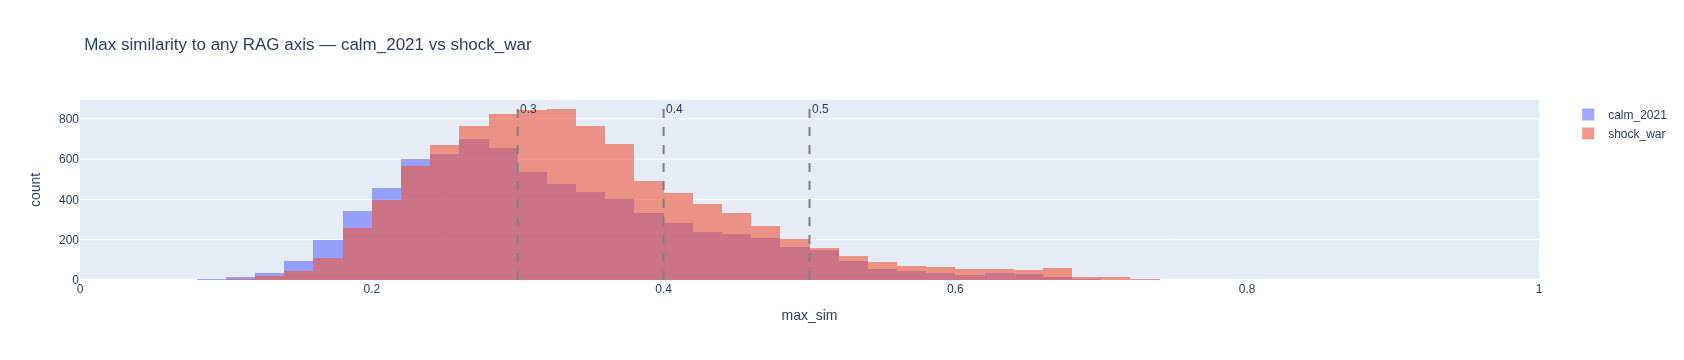
\includegraphics[width=\linewidth,height=0.46\textheight,keepaspectratio]{images/10_unimodal.png}

      \vspace{-4pt}
      {\small\color{BPMuted}
      «максимальная схожесть с любой из 9 осей — спокойный период vs санкционный шок»}
    \end{column}

    \begin{column}{0.38\textwidth}
      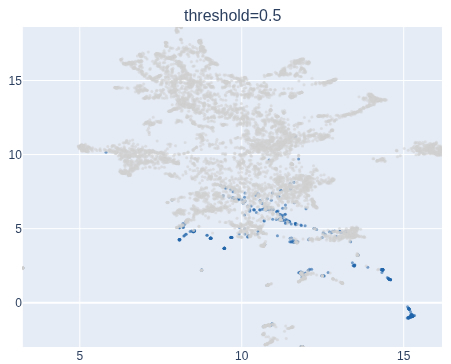
\includegraphics[width=\linewidth,height=0.46\textheight,keepaspectratio]{images/10_retr_vs_nonretr.jpg}

      \vspace{-4pt}
      {\small\color{BPMuted}
      «спокойный период, threshold=0.5 — retrieved (синий) vs остальные»}
    \end{column}
  \end{columns}

  \vspace{8pt}

  {\small\color{BPMuted}
  • распределение унимодальное — естественной границы сигнал/шум нет\\
  • при threshold=0.5 спокойный период почти пустой\\
  • решение: top-K=50 по каждой оси, prime1 исключён}
\end{frame}
